\documentclass[10pt, a4paper]{article}
\usepackage[a4paper, top=20mm, left=18mm, right=18mm, bottom=20mm]{geometry}
\usepackage{hyperref}
\usepackage[sf]{titlesec}
\usepackage{listings}
\usepackage{graphicx}
\usepackage{float}
\usepackage{color}
\hypersetup{hidelinks = true}
\definecolor{codegrey}{rgb}{0.95, 0.95, 0.96}
\lstset{backgroundcolor = \color{codegrey}}

\begin{document}
{\fontfamily{cmss}\selectfont

\title{\vspace{-20mm}CMPUT 291 - Mini Project 1 Design Document}
\date{}
\maketitle
\vspace{-20mm}
\section{Overview}\label{OV}
The following python application is used to connect to an existing SQLite3 database storing enterprise data. The application is run through the terminal, and is operated with simple command line inputs. For information on connecting to a database and running the application, see \emph{\nameref{UG}}.

Users with valid login credentials will be provided access to various functions to interact, view, and update the data stored in the database. Depending on their user type (determined by the database) the functionalities include: \emph{Register a birth, Register a marriage, Renew a vehicle registration, Process a bill of sale, Process a payment, Get a driver abstract, Issue a ticket, Find a car owner}. For specifics on these functions and their operations, see \emph{\nameref{SD}}.

\subsection{User Guide}\label{UG}
To launch the application, run the following command from the directory holding the source code:
\begin{lstlisting}
    $ python3 db.py
\end{lstlisting}
To connect to a database, enter the path to the database when prompted (a):
\begin{lstlisting}
    Enter path of database: path/to/database.db
\end{lstlisting}
Once the database connection is successfully established, the user will be prompted to enter their username and password (b), for example:
\begin{lstlisting}
    Username: admin123
    Password: pwd12345
\end{lstlisting}
Depending in the user type (agent or officer), numerical options will appear on screen. Enter the number of the task you wish to perform, and follow the on-screen instructions. For further information regarding the options, see \emph{\nameref{SD}}. 

At the main user menu, the user can logout by entering the `0' key, which will return the application to the login screen. The application will remain connected to the database entered at launch, and other users are able to login from here.

The user can return to the main menu from any point within performing a task by hitting ctrl-d. Note: if a new entity was committed to the database or before hitting crtl-d, \textbf{this action will be saved in the database}, i.e. if a parent needs to be registered in order to register a birth, and this step is completed, and the user exits to the main menu before completing the birth registration process, the newly registered parent will remain in the database. 

At the login in screen, the application can be exited by pressing crtl-d.

\begin{figure}[H]
\centering
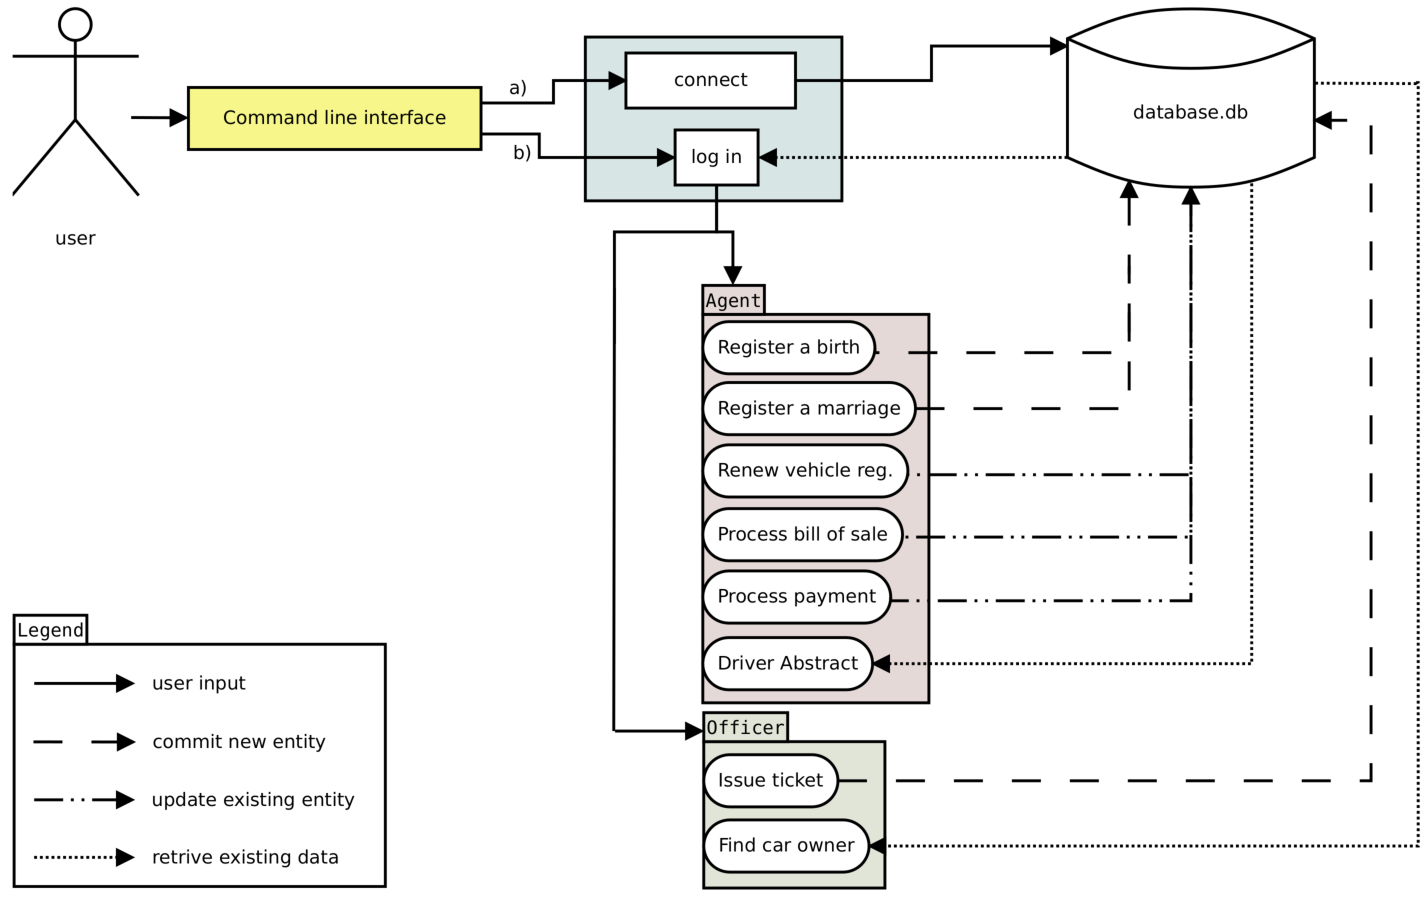
\includegraphics[height=8cm]{Diagram1.pdf}\label{fig}
\caption{Diagram showing flow of data between application user, application functions, and the connected database.}
\end{figure}

\section{Software Design}\label{SD}
\begin{itemize}

\item User Menu [\texttt{display\_menu(utype)}]
	\begin{quotation}
	\noindent After a successful log in, the user is provided a menu with an enumerated list of tasks they can perform, depending on their \texttt{utype}. By entering the number corresponding to a task and hitting the ENTER key, the program will display a new page with on-screen inputs and instructions on how to complete the task.
	\end{quotation}

\item Register a person [\texttt{insert\_person(fname, lname)}]
	\begin{quotation}
	\noindent Registers a new person into \emph{persons} table. If \texttt{fname, lname} are not provided as arguments, user can enter this information. Otherwise, names provided as arguments will be used. 
	\end{quotation}
	
\item Register a birth [\texttt{register\_birth(user\_info)}]
	\begin{quotation}
	\noindent Registers a new person into \emph{persons} table and a new birth record in \emph{births} table with a unique registration number generated by the program. Prompts user to enter child's first and last name, birth gender, mother's first and last name, father's first and last name, and the child's birth date and birth place. Registration place is automatically set to the user's city (from \texttt{user\_info}), and registration date is set to today's date. Child inherits mother's address and phone number, which is obtained from a query within the function. In the case where the mother or father do not exist in the database, the user has the option to register them, which calls \texttt{insert\_person(fname, lname)}
	\end{quotation}
	
\item Register a marriage [\texttt{register\_marriage(user\_info)}]
	\begin{quotation}
	\noindent Registers a new marriage record; registration numbers automatically generated by the program. User enters both partners first and last name. If partner is not found in database, user can register them first, calling \texttt{insert\_person(fname, lname)}. Registration place is determined by \texttt{user\_info}, and date is set to today's date. 
	\end{quotation}
	
\item Renew a vehicle registration [\texttt{renew\_reg()}]
	\begin{quotation}
	\noindent Receives a registration number from user input, then sets the registration date to the current date and the expiry to be one year after.
	\end{quotation}

\item Process a bill of sale [\texttt{bill\_of\_sale()}]
	\begin{quotation}
	\noindent Prompts user to enter a vin, current and new owner for a vehicle, the creates a registration for the new owner. The system also expires the old registration. The system allows the user to re-enter any incorrect information.
	\end{quotation}

\item Process a payment [\texttt{process\_payment()}]
	\begin{quotation}
	\noindent Receives a ticket number and payment amount from the user. The system records the payment into the database. The user is not allowed to enter a payment amount that will exceed what is due on the ticket.
	\end{quotation}

\item Get a driver abstract [\texttt{get\_driver\_abstract()}]
	\begin{quotation}
	\noindent Prompts user to enter first and last name of a registered person to display their driver abstract. If the name entered is not found, the user has the option to renter the name, or return to the main menu. The driver abstract consists of: ticket counts for lifetime and last two years, demerit notices and points for lifetime and last two years. The agent has the option to view a detailed ticket history by entering the t/T key. Initially five tickets are displayed in order from most recent to oldest, with an option to display 5 more until the end of the history.
	\end{quotation}

\item Issue a ticket [\texttt{issue\_ticket()}]
	\begin{quotation}
	\noindent Creates a new ticket entry in \emph{tickets} table. User will be asked to enter a valid registration number; if number is invalid user will be returned to menu. If a valid registration number is entered, registration details are displayed to the user. From here, they enter violation date (defaults to today's date if field left blank), description, and fine amount. A unique ticket number is generated by the program by taking the largest existing number and incrementing it by one. 
	\end{quotation}
\newpage
\item Find a car owner [\texttt{find\_car\_owner()}]
	\begin{quotation}
	\noindent Prompts user to optionally enter the make, model, year, colour and plate of a vehicle. Matching vehicles are found and displayed with their make, model, year, colour and plate. The user may choose a vehicle to view the registration date, expiry date and the name of the owner. Alternatively, if there are less than 3 matches the additional information is displayed automatically.
	\end{quotation}

\end{itemize}

\section{Testing Strategy}\label{TS}
Functions of the software were tested as they were developed, and then again when the entire development process was completed. For each of the functionalities, the following cases were tested:
\begin{itemize}
\item{\emph{Register a birth}: Both parents in db; only one parent in db; no parents in db; mother with Null values}
\item{\emph{Register a marriage}: partners not in db}
\item{\emph{Renew a vehicle registration}: regno not found}
\item{\emph{Process a bill of sale}: regno, current and/or new owner not in db}
\item{\emph{Process a payment}: invalid tno; invalid payment amount (i.e. over paying a ticket)}
\item{\emph{Get a driver abstract}: driver not found in db}
\item{\emph{Issue a ticket}: regno not found; violation date specified; violation date not specified }
\item{\emph{Find a car owner}: No info entered, less than 4 results, more than 4 results}
\end{itemize}

\section{Group Break-down Strategy}\label{GS}
The project was developed using github to track progress and coordinate work on implementing the features outlined in the spec. A detailed breakdown of the group work on functions and features follows: 
	
	\begin{itemize}
	\item main, database connection, user login, main menu [\texttt{main()/connect\_to\_DB()/get\_login()/display\_menu(utype)}]
		\begin{itemize}
		\item Dalton \& Harrison: collaborative, 1.5 hrs
		\end{itemize}
		
	\item SQL injection prevention and non-visible password
		\begin{itemize}
		\item Harrison \& Dalton: collaborative, 0.5 hrs
		\end{itemize}
	
	\item Register a birth [\texttt{register\_birth(user\_info)/insert\_person()}]
		\begin{itemize}
		\item Harrison \& Dalton: collaborative, 1 hrs
		\end{itemize}
	
	\item Register a marriage [\texttt{register\_marriage(user\_info)}]
		\begin{itemize}
		\item Harrison \& Dalton: collaborative, 0.5 hrs
		\end{itemize}

	\item Renew a vehicle registration [\texttt{renew\_reg()}]
		\begin{itemize}
		\item Harrison \& Dalton: collaborative, 0.5 hrs
		\end{itemize}
		
	\item Bill of sale [\texttt{bill\_of\_sale()}]
		\begin{itemize}
		\item Amir: 2 hrs
		\item Harrison: format changes, 0.5 hours
		\end{itemize}
		
	\item Process a payment [\texttt{process\_payment()}]
		\begin{itemize}
		\item Harrison \& Dalton \& Amir: collaborative, 1 hrs
		\end{itemize}
		
	\item Get a driver abstract [\texttt{get\_driver\_abstract()/ticket\_report()}]
		\begin{itemize}
		\item Dalton: 3 hrs
		\end{itemize}
		
	\item Issue a ticket [\texttt{issue\_ticket()}]
		\begin{itemize}
		\item Harrison \& Dalton \& Amir: collaborative, 1 hrs
		\end{itemize}
		
	\item Find a car owner [\texttt{find\_car\_owner()}]
		\begin{itemize}
		\item Amir: 8 hours
		\item Harrison \& Dalton \& Amir: collaborative, 1.5 hrs
		\end{itemize}
	
	\item ctrl-d escape
		\begin{itemize}
		\item Harrison: 1 hrs
		\end{itemize}	
	
	\item Design Document
		\begin{itemize}
		\item Dalton: format, flow diagram, overview, user guide, 3 hrs
		\item Harrison \& Dalton \& Amir: collaborative, 1.5 hrs
		\end{itemize}
	\end{itemize}

\end{document}
